\section{Anexos} \label{sec:anexo}
	\subsection{Imagens do Carro Montado}

		\begin{figure}[h]
			\centering
			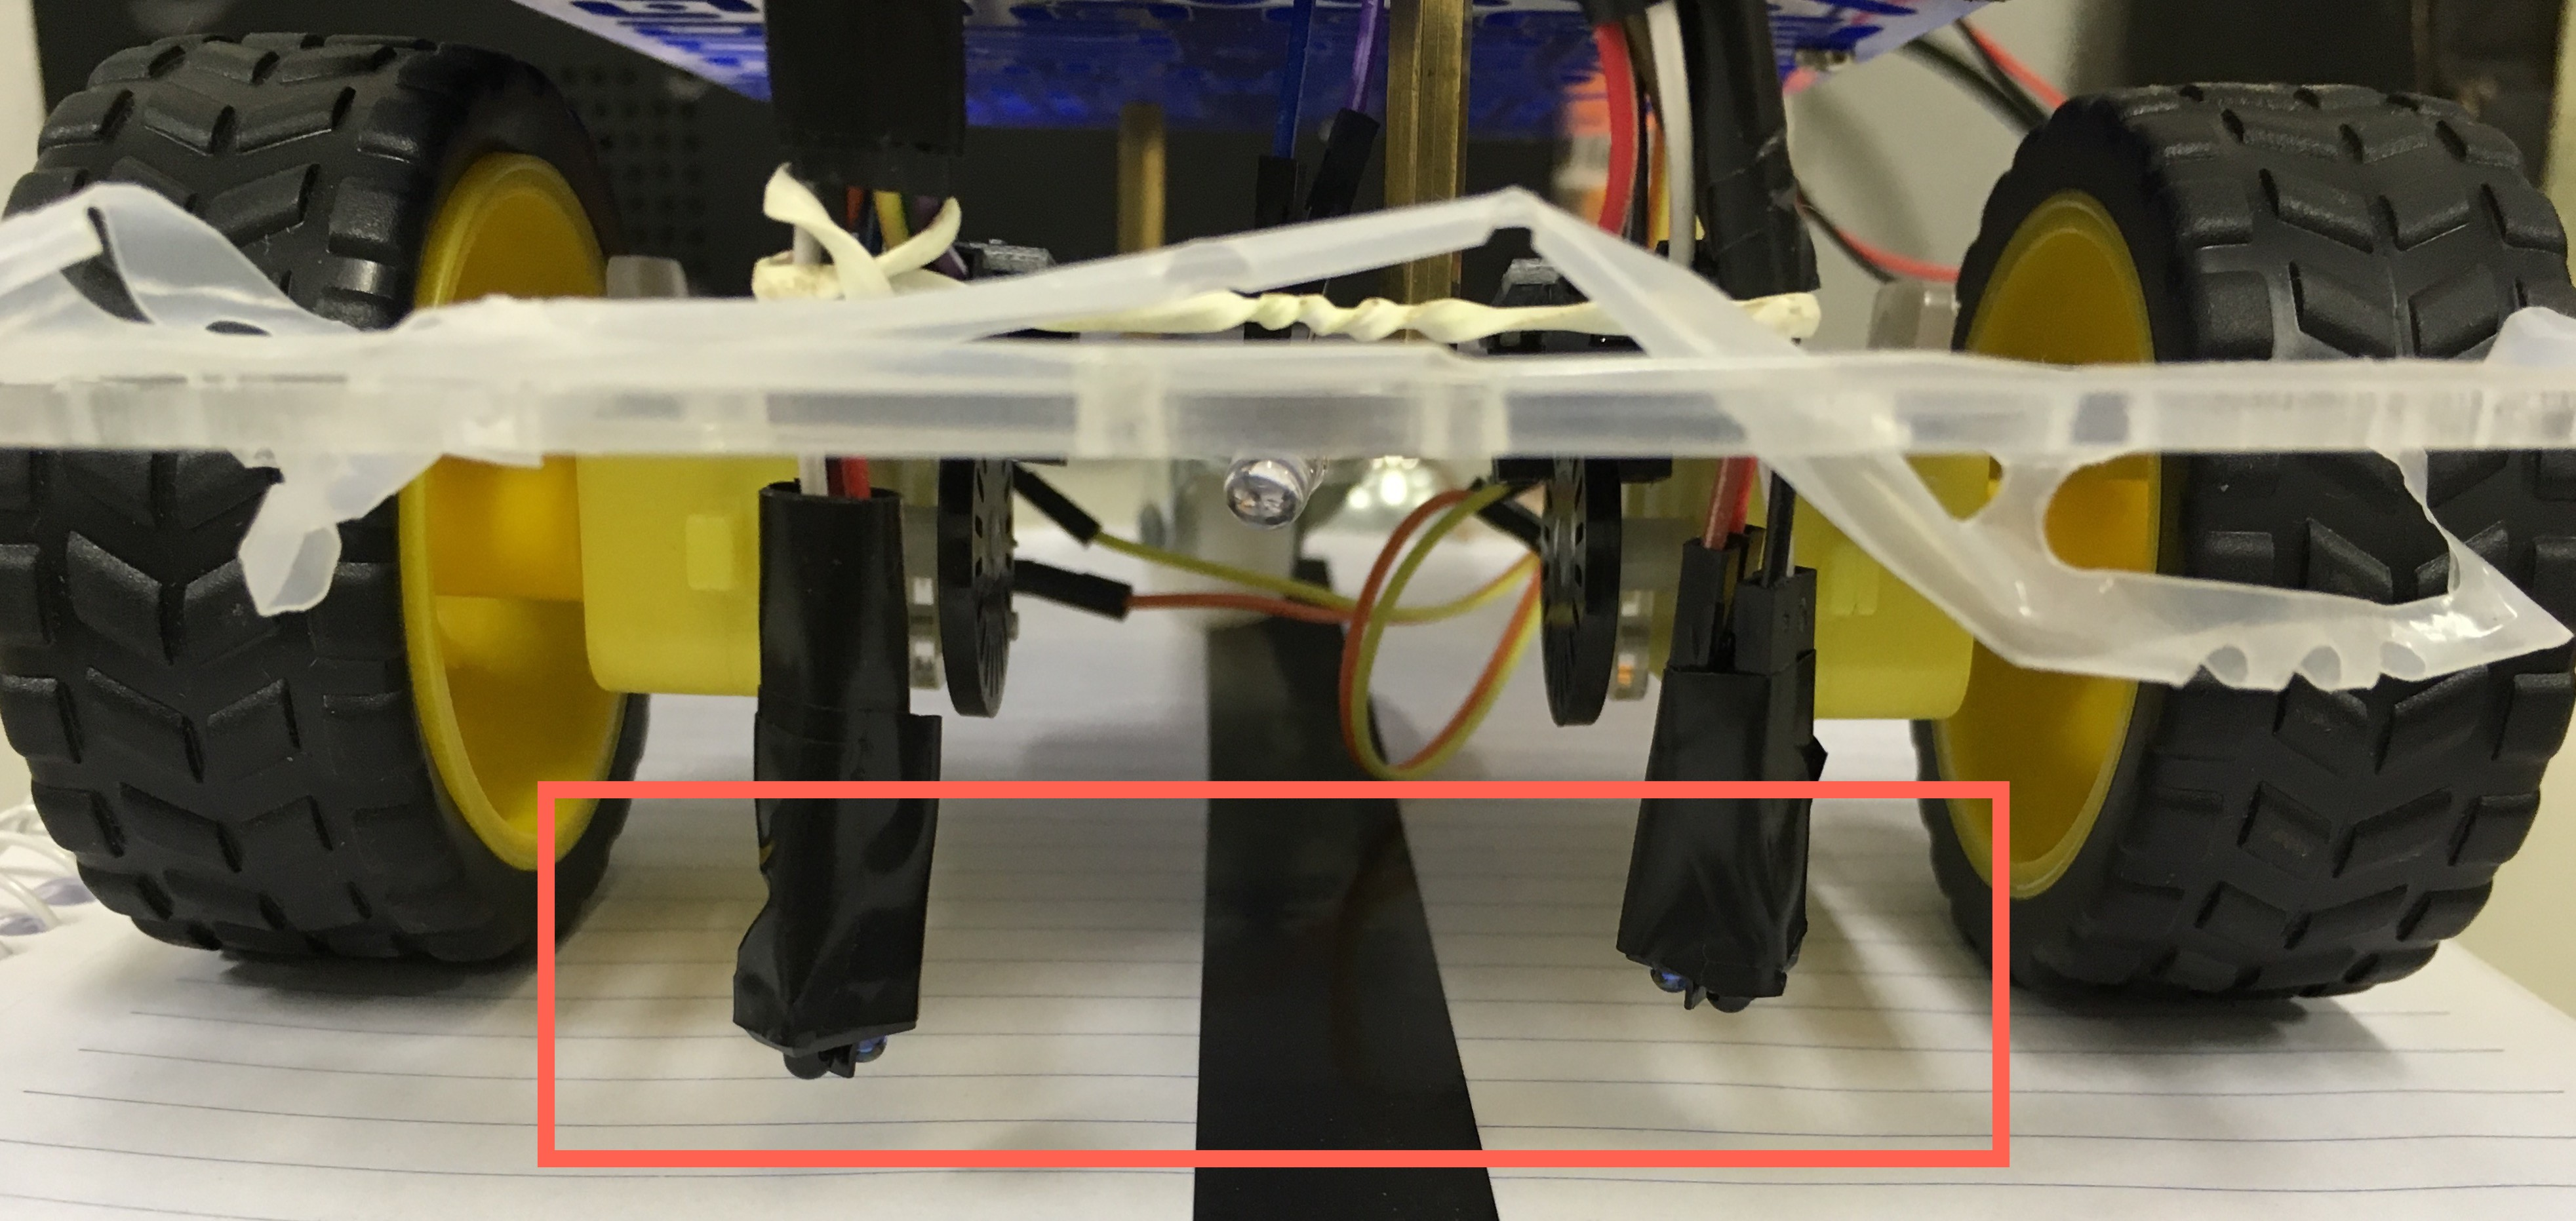
\includegraphics[width=1\linewidth]{img/robot_fotos.jpg}
			\label{fig:robot_foto}
			\caption{Carro Robô $ \mathcal{A} $ e os sensores fototransistores.}
		\end{figure}

		\begin{figure}[h]
			\centering
			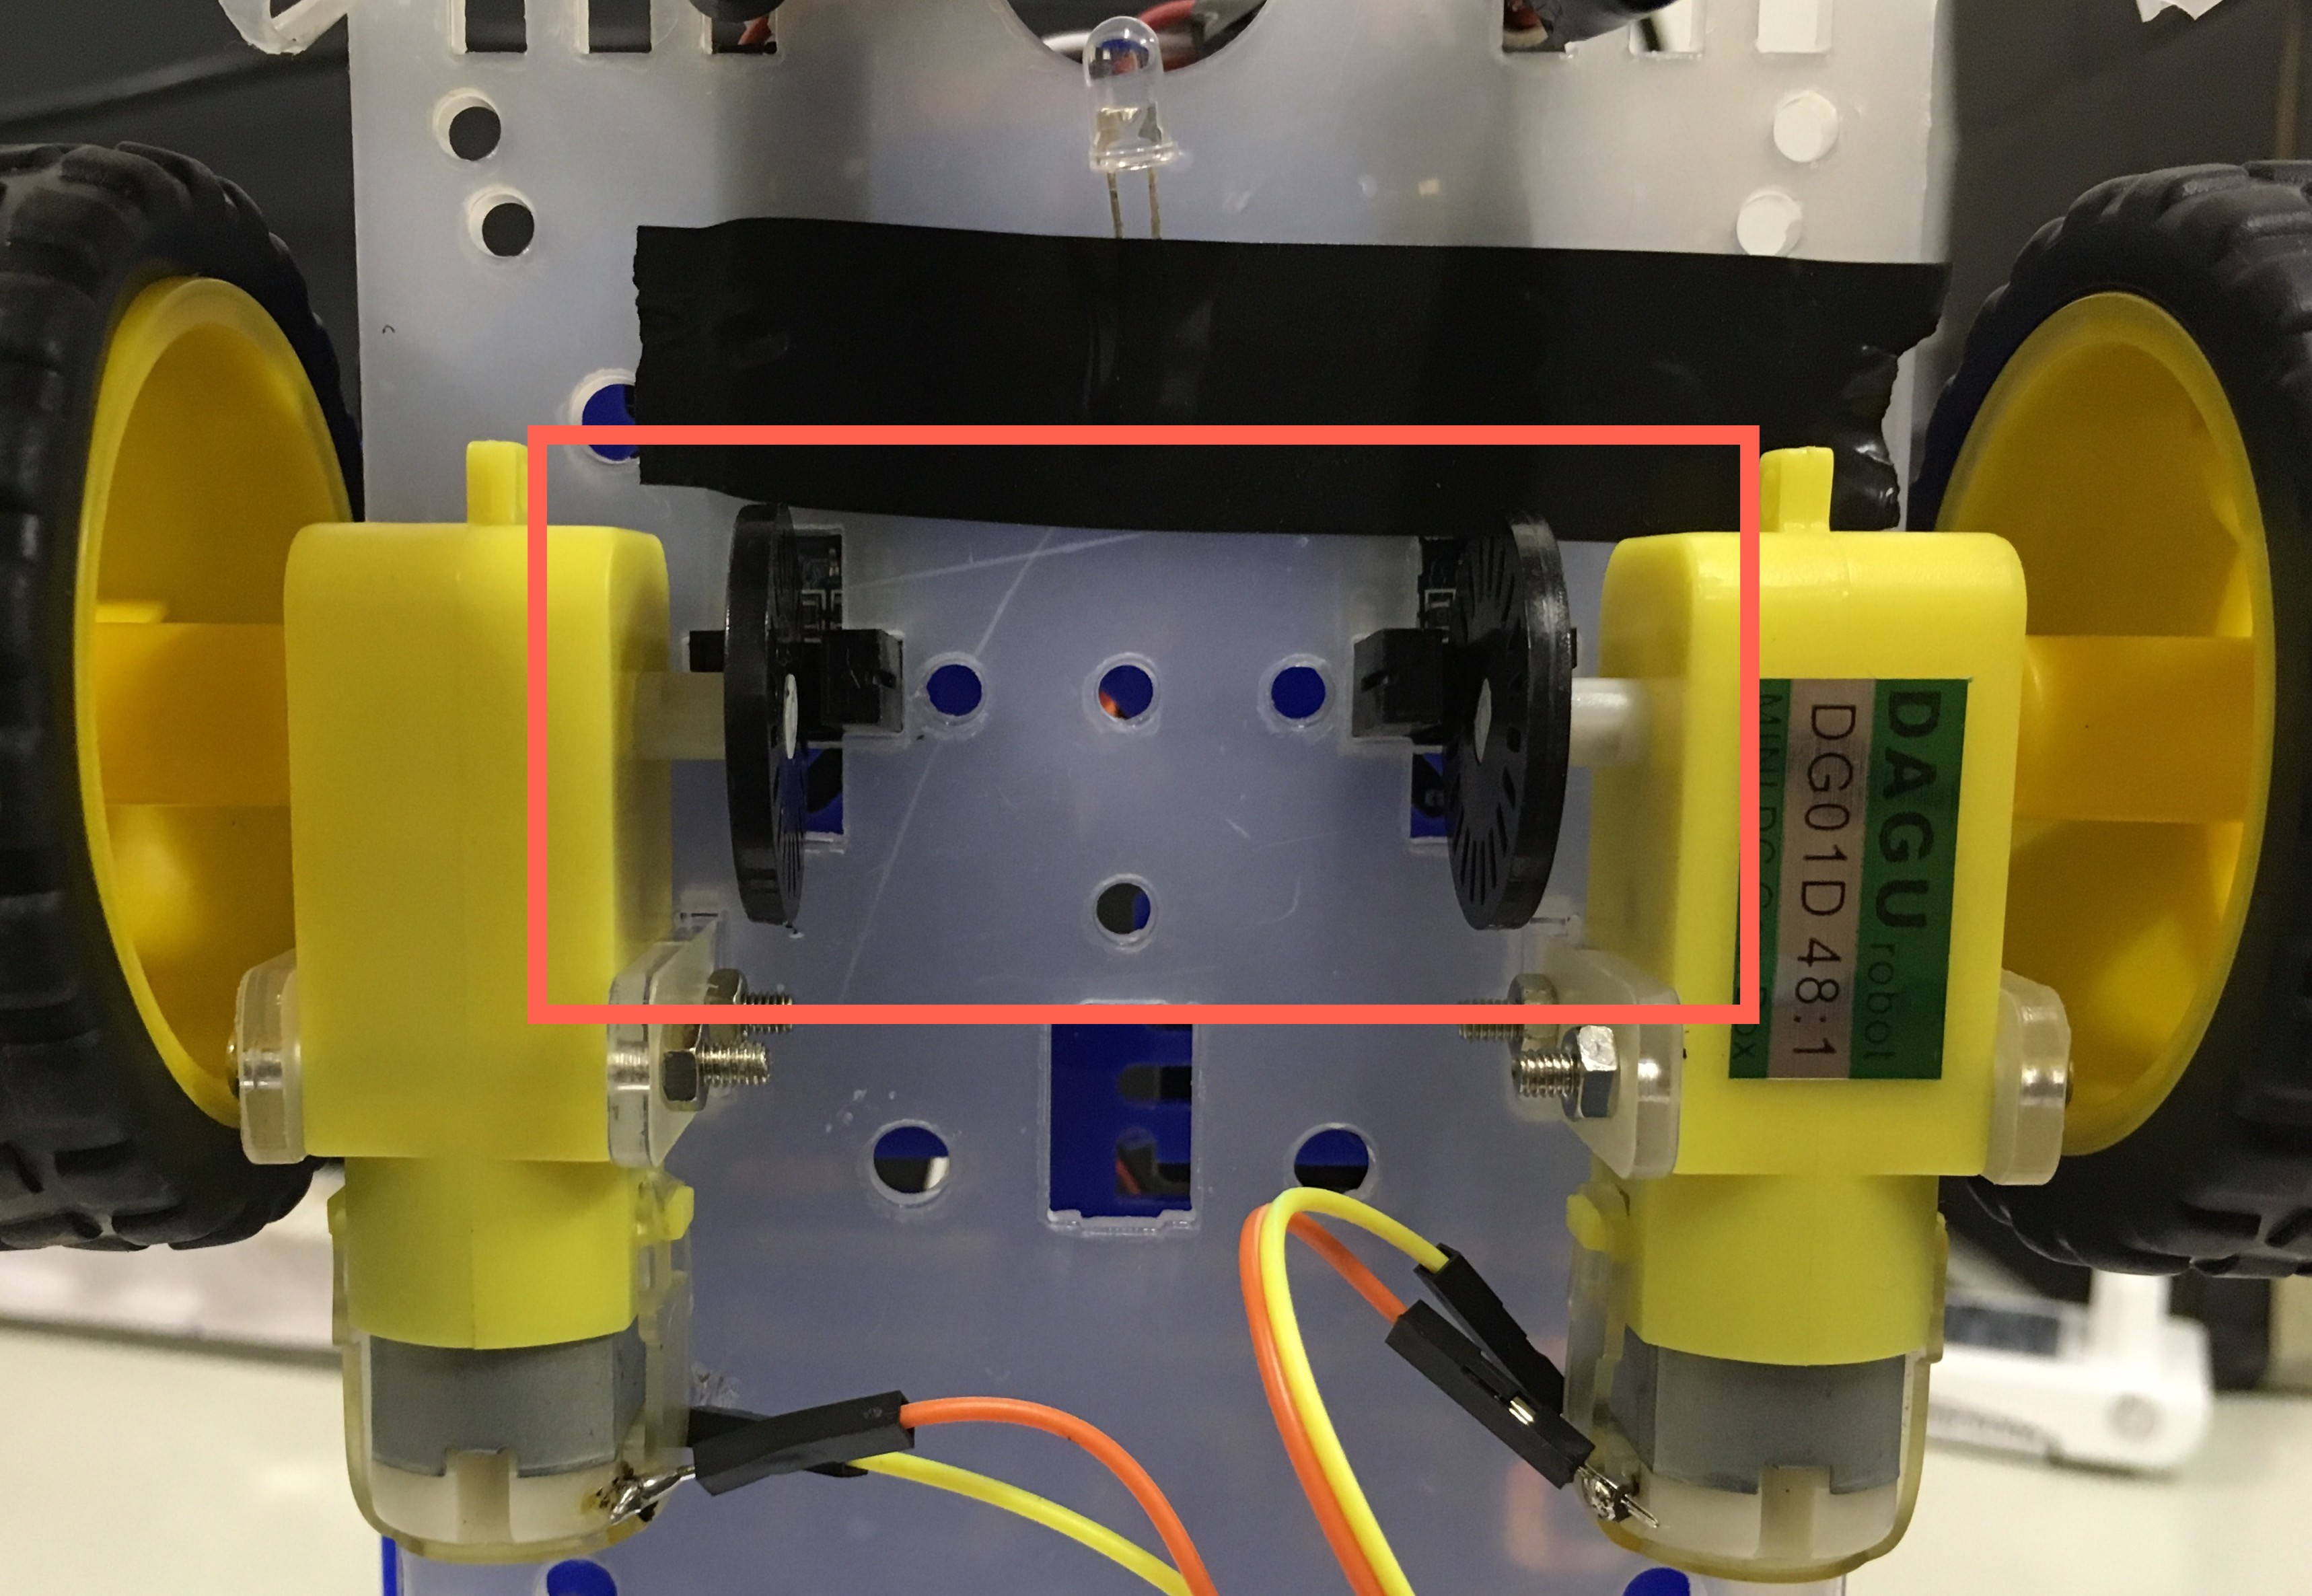
\includegraphics[width=1\linewidth]{img/robot_encoders.jpg}
			\label{fig:robot_encoder}
			\caption{Carro Robô $ \mathcal{A} $ e os sensores encoders.}
		\end{figure}
        
		\begin{figure}[ht]
			\centering
			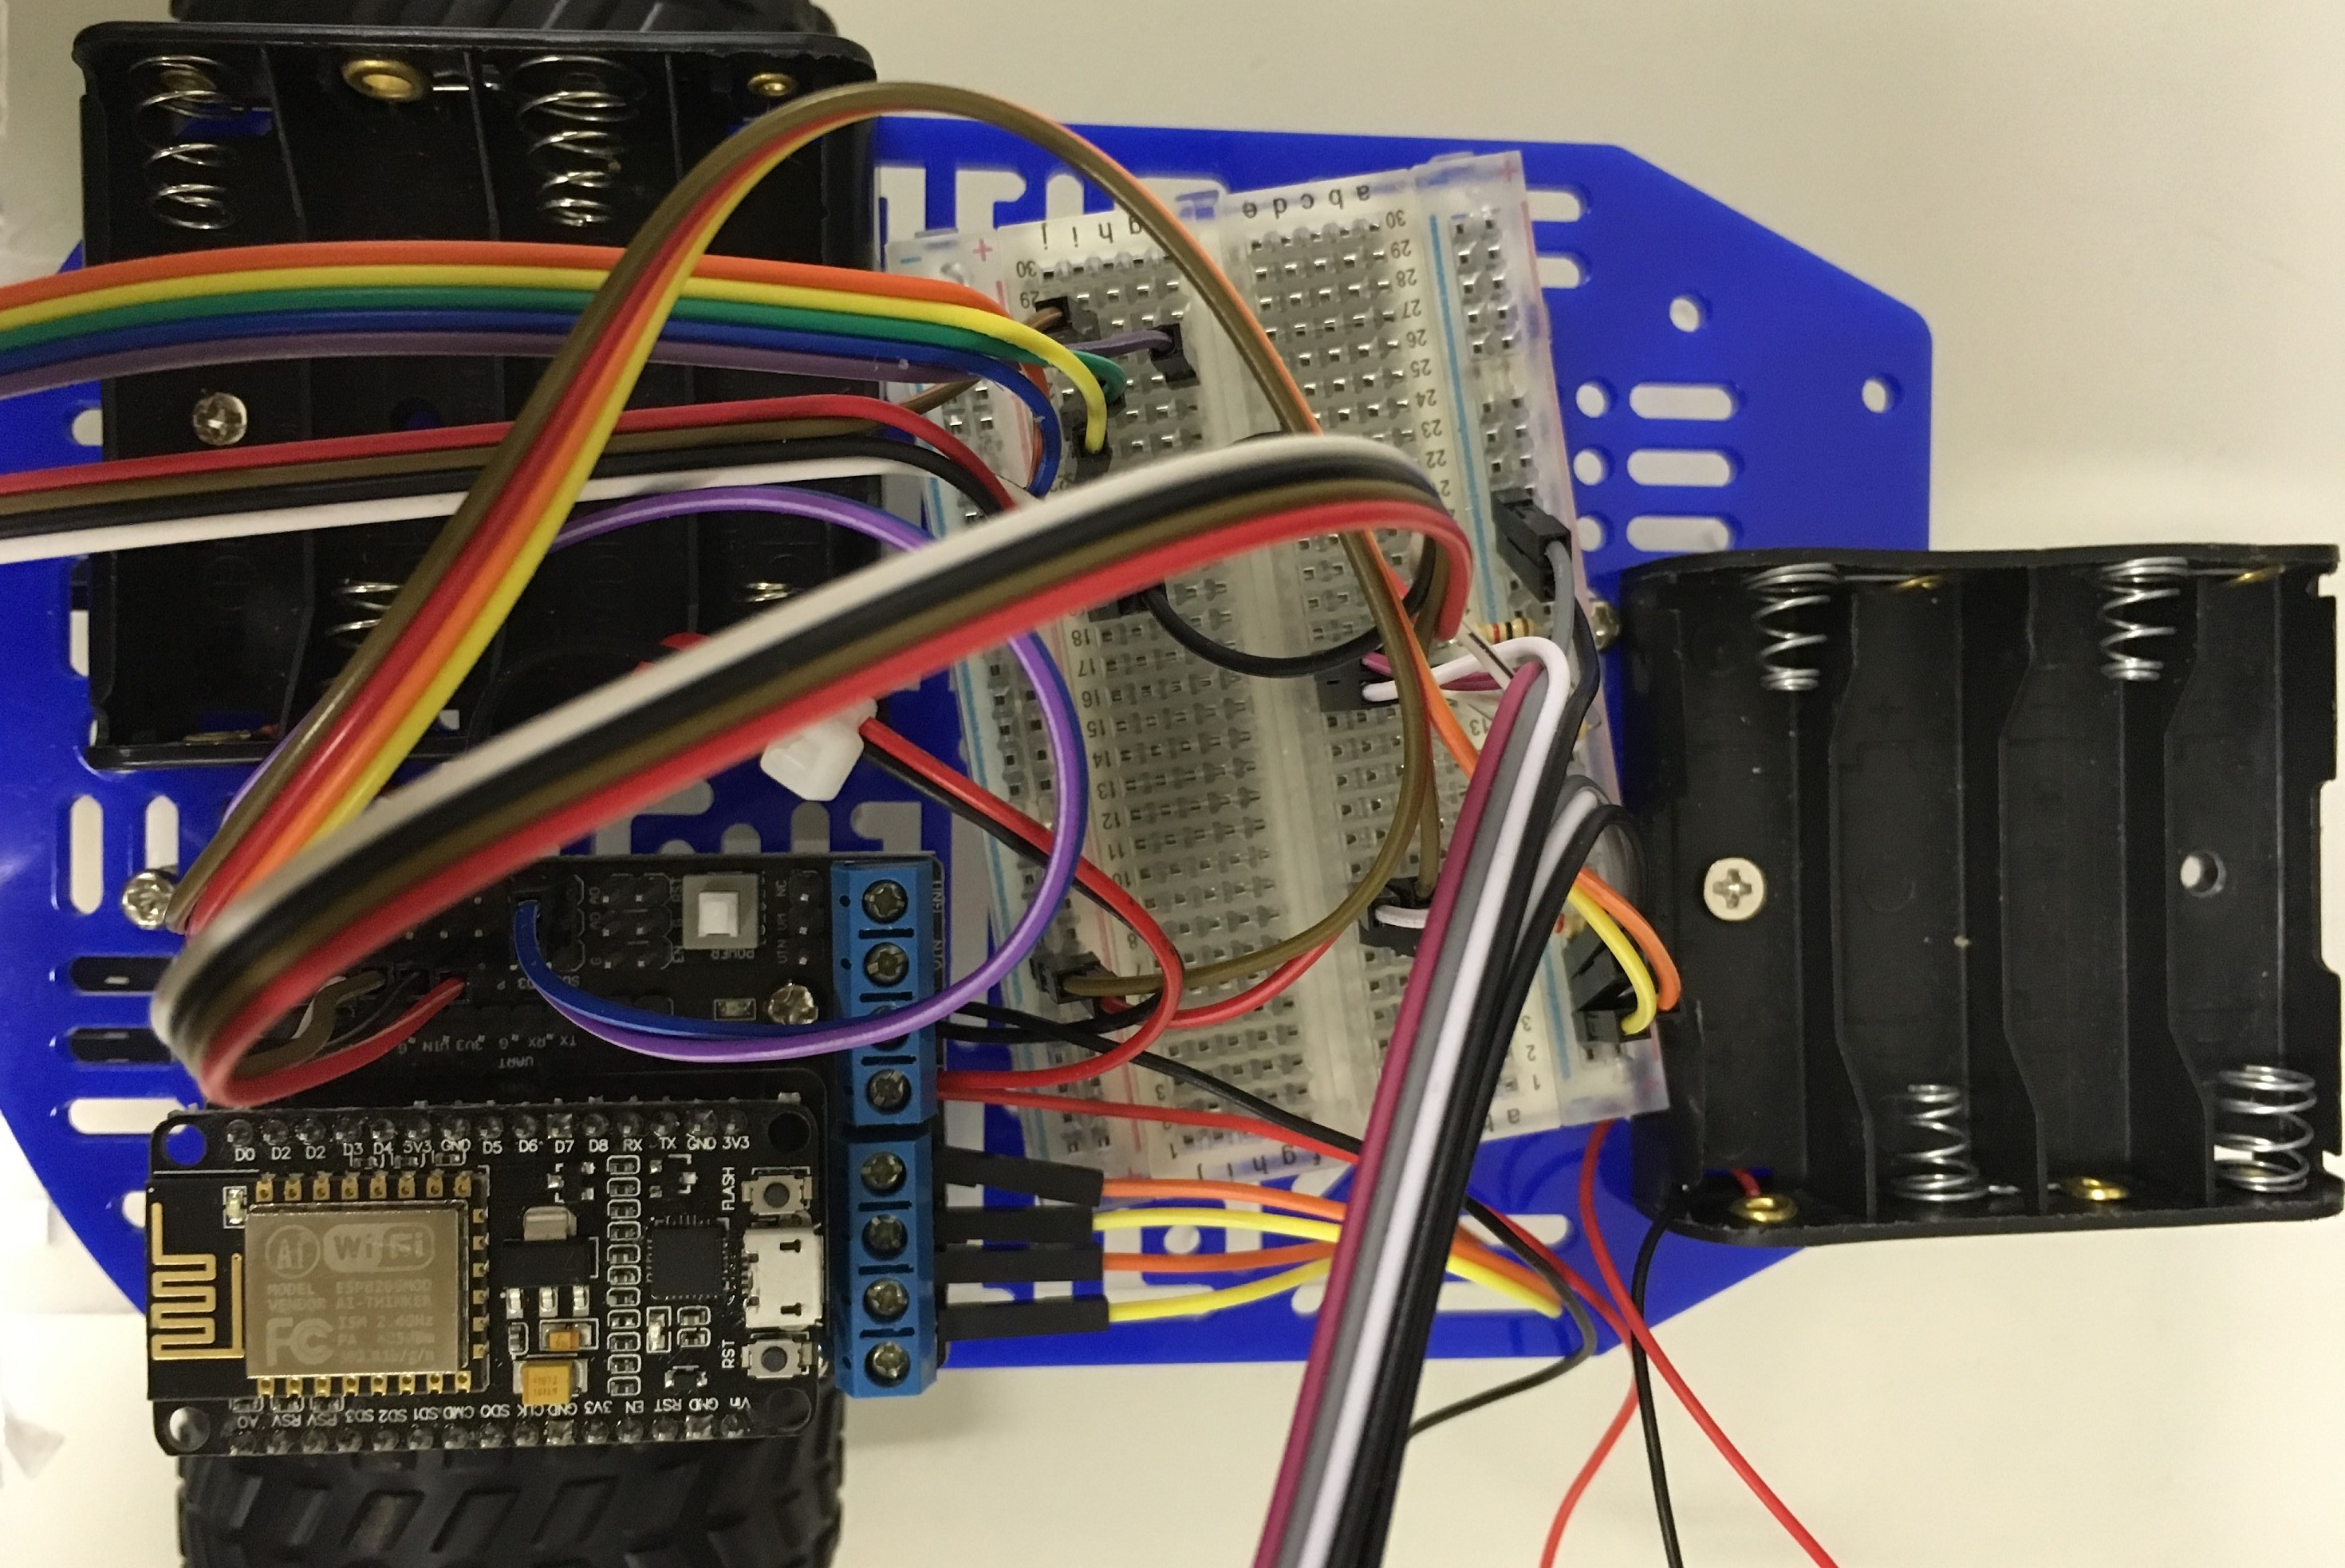
\includegraphics[width=1\linewidth]{img/robot.jpg}
			\label{fig:robot}
			\caption{Carro Robô $ \mathcal{A} $.}
		\end{figure}
		
	\subsection{Código em Linguagem Arduino}
	\subsubsection{ploudy NodeMCU}
		\begin{minted}
			[
			frame=lines,
			framesep=2mm,
			tabsize=3,
			breaklines=true,
			baselinestretch=1.2,
			fontsize=\scriptsize,
			linenos
			]{c++}
#include <SoftwareSerial.h>
#include <stdio.h>
#include <ESP8266WiFi.h>
#include <Wire.h>
#include "MPU9250.h"



// =============== Constants ===================================
#define RADIUS        3.4
#define LARGURE       13.42
#define NUMBER_FRAMES 40
#define DELTA_TEMPO   75
#define SERIALDEBUG   true        
#define SSID          "Imobilis"
#define SSID_PASSWORD "bolinha de sabao"
#define URL           "192.168.0.174"
#define PORT          8888

// =============== Instantiations ==============================
WiFiClient client;
MPU9250 accelgyro;
I2Cdev   I2C_M;
// =============== Variables for MPU9250 =======================
#define sample_num_mdate  5000
volatile float mx_sample[3], my_sample[3], mz_sample[3];
static float mx_centre = 0, my_centre = 0, mz_centre = 0;
static float mx_max = 0, my_max = 0, mz_max = 0;
static float mx_min = 0, my_min = 0, mz_min = 0;
uint8_t buffer_m[6];
int16_t mx, my, mz;
float heading;
float Mxyz[3];
// =============== Human Interface and Controls ================
char command         = '0';
bool restart_program = true;
// =============== Pins ========================================
long pin_left_motor_pwm           = D1;  // Pin to left motor pwm          
long pin_righ_motor_pwm           = D2;  // Pin to righ motor pwm          
long pin_left_motor_pwm_direction = D3;  // Pin to left motor direction
long pin_righ_motor_pwm_direction = D4;  // Pin to righ motor direction
long pin_left_optical_sensor      = D5;  //Pin to optical sensor
long pin_righ_optical_sensor      = D6;  //Pin to optical sensor
long left_encoder                 = D7;  // Pin to encoder
long righ_encoder                 = D8;  // Pin to encoder
// =============== Timing ========================
unsigned long tempo               = 0;
unsigned long global_start_time   = 0;
unsigned long global_spended_time = 0;
// =============== Send Datas =================
byte left_light_boolean = 1, righ_light_boolean = 1;
byte left_light_boolean_inter = 1, righ_light_boolean_inter = 1;
// =============== Receive Datas =================
long size_map       = 0;
char s_package[256] ;
bool package_sent   = false;
String str_send     = "";

//TODO: Rever essas variáveis se estão postas de forma certa
int left_master_pwm    = 0;
int righ_master_pwm    = 0;
int left_master_frames = 0;
int righ_master_frames = 0;

// =============== Encoder Angular Velocity ====================
long left_current_encoder_this_car = 0;
long righ_current_encoder_this_car = 0;
long left_last_encoder_this_car    = 0;
long righ_last_encoder_this_car    = 0;
long x_point                       = 0;
long y_point                       = 0;
int reference                      = 0;




 float calculating_heading(void) {
	heading = 180 * atan2(Mxyz[1], Mxyz[0]) / PI;
	if (heading < 0) heading += 360;

	return heading;
}

void getTiltHeading(void) {
	float pitch = asin(-Axyz[0]);
	float roll = asin(Axyz[1] / cos(pitch));

	float xh = Mxyz[0] * cos(pitch) + Mxyz[2] * sin(pitch);
	float yh = Mxyz[0] * sin(roll) * sin(pitch) + Mxyz[1] * cos(roll) - Mxyz[2] * sin(roll) * cos(pitch);
	float zh = -Mxyz[0] * cos(roll) * sin(pitch) + Mxyz[1] * sin(roll) + Mxyz[2] * cos(roll) * cos(pitch);
	tiltheading = 180 * atan2(yh, xh) / PI;
	if (yh < 0)    tiltheading += 360;
}


void Mxyz_init_calibrated () {
	Serial.print("\n[INFO] Sample starting......");  
	Serial.print("\n[INFO] waiting ......");

	get_calibration_Data ();

	Serial.print("[INFO] Compass calibration parameter: ");
	Serial.print(mx_centre); Serial.print(", ");
	Serial.print(my_centre); Serial.print(", ");
	Serial.print(mz_centre);
}


void get_calibration_Data () {

	get_one_sample_date_mxyz();
	mx_max = mx_sample[2];
	my_max = mx_sample[2];
	mz_max = mx_sample[2];
	mx_min = mx_sample[2];
	my_min = mx_sample[2];
	mz_min = mx_sample[2];

	for (int i = 0; i < sample_num_mdate; i++) {
		get_one_sample_date_mxyz();

		Serial.print("\n");
		Serial.print(i); Serial.print(":");
		Serial.print(sample_num_mdate); Serial.print("   ");
		Serial.print(mx_sample[2]); Serial.print(" ");
		Serial.print(my_sample[2]); Serial.print(" ");
		Serial.print(mz_sample[2]);

		if (mx_sample[2] >= mx_max) mx_max = mx_sample[2];
		if (my_sample[2] >= my_max) my_max = my_sample[2];
		if (mz_sample[2] >= mz_max) mz_max = mz_sample[2];
		if (mx_sample[2] <= mx_min) mx_min = mx_sample[2];
		if (my_sample[2] <= my_min) my_min = my_sample[2];
		if (mz_sample[2] <= mz_min) mz_min = mz_sample[2];

	}
	mx_centre = (mx_max + mx_min) / 2;
	my_centre = (my_max + my_min) / 2;
	mz_centre = (mz_max + mz_min) / 2;
}

void get_one_sample_date_mxyz() {
	getCompass_Data();
	mx_sample[2] = Mxyz[0];
	my_sample[2] = Mxyz[1];
	mz_sample[2] = Mxyz[2];
}

void getCompass_Data(void) {
	I2C_M.writeByte(MPU9150_RA_MAG_ADDRESS, 0x0A, 0x01); //enable the magnetometer
	delay(10);
	I2C_M.readBytes(MPU9150_RA_MAG_ADDRESS, MPU9150_RA_MAG_XOUT_L, 6, buffer_m);

	mx = ((int16_t)(buffer_m[1]) << 8) | buffer_m[0] ;
	my = ((int16_t)(buffer_m[3]) << 8) | buffer_m[2] ;
	mz = ((int16_t)(buffer_m[5]) << 8) | buffer_m[4] ;

	Mxyz[0] = (double) mx * 1200 / 4096;
	Mxyz[1] = (double) my * 1200 / 4096;
	Mxyz[2] = (double) mz * 1200 / 4096;
}

void getCompassDate_calibrated () {
	getCompass_Data();
	Mxyz[0] = Mxyz[0] - mx_centre;
	Mxyz[1] = Mxyz[1] - my_centre;
	Mxyz[2] = Mxyz[2] - mz_centre;
}


float get_heading() {
    getCompassDate_calibrated();
    return calculating_heading();
}


//          10-DOF
// ===================================================================================================================
// ===================================================================================================================
//          PROCEDIMENTOS ENCODER


int difference_trick_encoder_left() { 
	int diff = left_current_encoder_this_car - left_last_encoder_this_car; 

	if (diff > 8) 
		diff = 0;

	left_last_encoder_this_car = left_current_encoder_this_car;
	return diff;
}
int difference_trick_encoder_righ() { 
	int diff = righ_current_encoder_this_car - righ_last_encoder_this_car; 

	if (diff > 8) 
		diff = 0;

	righ_last_encoder_this_car = righ_current_encoder_this_car;
	return diff;
}

float left_distance_centimeters() { return 2 * PI * RADIUS * (difference_trick_encoder_left()) / NUMBER_FRAMES ; }
float righ_distance_centimeters() { return 2 * PI * RADIUS * (difference_trick_encoder_righ()) / NUMBER_FRAMES ; }

float center_distance_centimeters() { return (righ_distance_centimeters() + left_distance_centimeters()) / 2.0; }


float refresh_x_point() { x_point = x_point + center_distance_centimeters() * cos(reference);   return x_point; }
float refresh_y_point() { y_point = y_point + center_distance_centimeters() * sin(reference);   return y_point; }
float refresh_reference() { reference = righ_distance_centimeters() - left_distance_centimeters() /
 LARGURE;    return reference; }


//          DEFINIÇÕES DE VARIÁVEIS
// ===================================================================================================================
// ===================================================================================================================
//          CONEXÕES DE REDE


unsigned long millis_now() { return millis() - global_start_time; }

void left_add_encoder() { left_current_encoder_this_car++; }
void righ_add_encoder() { righ_current_encoder_this_car++; }

void left_interrupt_ligth() { left_light_boolean_inter = 1; }
void righ_interrupt_ligth() { righ_light_boolean_inter = 1; }

// Função para iniciar a Conexão com a rede WiFi
void start_connection_wifi() {
	bool twice = false;
	do {
		if (SERIALDEBUG && ! twice) {
			Serial.print("\n[INFO] Connecting in: ");
			Serial.print(SSID); 
		}

		WiFi.begin(SSID, SSID_PASSWORD); // connecta na Rede Wireless

		while (WiFi.status() != WL_CONNECTED) {
			if (SERIALDEBUG && ! twice) 
				Serial.print("\n\tNão Conectado na Rede WiFi");
			delay(200);
			twice = true;
		}

		if (SERIALDEBUG) {
			Serial.print("\n[INFO] Conectado na Rede: \n\t");  Serial.print(SSID);
			Serial.print(" | IP ");
			Serial.print(WiFi.localIP());
		}

	} while (WiFi.status() != WL_CONNECTED);
}

void master_connection_cloud() {
	bool twice = false;
	do {
		if (SERIALDEBUG && ! twice) {
			Serial.print("\n[INFO] Start Cloud Connecting");
			Serial.print("\n\tAddress: ");
			Serial.print(URL); 
			Serial.print(" : ");
			Serial.println(PORT); 

			Serial.print("\n[INFO] Getting Connection with the cloud");
		}

		// configure traged server and url
		if(client.connect(URL, PORT)) {
			twice = false;
			if (SERIALDEBUG && ! twice) {
				Serial.print("\n[INFO] Connection with the cloud stablished");
				Serial.print("\n[INFO] Sending the robot information Hi");
			}

			client.print("Hi From Master Robot\0");

		} else {
			if (SERIALDEBUG && ! twice)
				Serial.print("\n[ERRO] Failed!");
			twice = true;
		}

		if (SERIALDEBUG && ! twice)
			Serial.print("\n[INFO] Finnishing Cloud Connecting");

	} while (! client.connected());
}

void verify_lost_connection_wifi() {
	//if (SERIALDEBUG) 
	//  Serial.print("\n[INFO] Verifing if there is connection.");

	if (WiFi.status() != WL_CONNECTED || ! client.connected()) {
		Serial.print("\n[ERRO] Desconnected! Restarting Everything.");
		motor_action(0, 0);
		
		ESP.restart();
	}
}

void slave_connection_cloud() {
	bool twice = false;
	do {
		if (SERIALDEBUG && ! twice) {
			Serial.print("\n[INFO] Start Cloud Connecting");
			Serial.print("\n\tAddress: ");
			Serial.print(URL); 
			Serial.print(" : ");
			Serial.println(PORT); 

			Serial.print("\n[INFO] Getting Connection with the cloud");
		}

		// configure traged server and url
		if(client.connect(URL, PORT)) {
			twice = false;
			if (SERIALDEBUG && ! twice) {
				Serial.print("\n[INFO] Connection with the cloud stablished");
				Serial.print("\n[INFO] Sending the robot information");
			}

			client.print("Hi From Slave Robot\0");

		} else {
			if (SERIALDEBUG && ! twice)
				Serial.print("\n[ERRO] Failed!");
			twice = true;
		}

		if (SERIALDEBUG && ! twice)
			Serial.print("\n[INFO] Finnishing Cloud Connecting");

	} while (! client.connected());
}


//          CONEXÕES DE REDE
// ===================================================================================================================
// ===================================================================================================================
//          PACOTES DE ENVIO


void set_package_values(int &left_pwm, int &righ_pwm){
	left_light_boolean = (int) digitalRead(pin_left_optical_sensor) || left_light_boolean_inter;
	righ_light_boolean = (int) digitalRead(pin_righ_optical_sensor) || righ_light_boolean_inter;

	left_light_boolean_inter = 0;
	righ_light_boolean_inter = 0;

}

void create_string_values() {
	s_package[0] = '\0';

	str_send = "";
	str_send = str_send + " " + millis_now()+ "  " + left_light_boolean + " " + 
	righ_light_boolean + "  " + left_current_encoder_this_car + " " + righ_current_encoder_this_car;// + "  " + get_heading();

}

void prepare_and_send_new_datas(int &left_pwm, int &righ_pwm) {
	set_package_values(left_pwm, righ_pwm);
	create_string_values();

	if (client.connected())
		client.print(str_send);
	else
		ESP.restart();
}


//          PACOTES DE ENVIO
// ===================================================================================================================
// ===================================================================================================================
//          PACOTES DE RECEBIMENTO



void get_new_values_master(int &left_pwm, int &righ_pwm) {
	char * left_motor_pwm_token;
	char * righ_motor_pwm_token;
	const char search[2] = " ";
	
	left_motor_pwm_token    = strtok(s_package, search);
	righ_motor_pwm_token    = strtok(NULL, search);

	left_pwm = atoi(left_motor_pwm_token);
	righ_pwm = atoi(righ_motor_pwm_token);
}

void get_new_values_slave() {
	char * tempo_token;
	char * left_master_pwm_token;
	char * righ_master_pwm_token;
	char * left_master_frames_token;
	char * righ_master_frames_token;
	const char search[2] = " "; 

	tempo_token                   = strtok(s_package, search);
	left_master_pwm_token         = strtok(NULL, search);
	righ_master_pwm_token         = strtok(NULL, search);
	left_master_frames_token      = strtok(NULL, search);   
	righ_master_frames_token      = strtok(NULL, search);  

	tempo                   = atoi(tempo_token);
	left_master_pwm         = atoi(left_master_pwm_token);
	righ_master_pwm         = atoi(righ_master_pwm_token);
	left_master_frames      = atoi(left_master_frames_token);
	righ_master_frames      = atoi(righ_master_frames_token);
}

void motor_action(long left_velocity, long righ_velocity) {
	long max = 1023;

	Serial.printf("\nL:%d %d\n", left_velocity, righ_velocity);

	if (left_velocity > 0) {
		digitalWrite(pin_left_motor_pwm_direction,  HIGH);
		if (left_velocity > max) {
			left_velocity = max;
		}    
	
	}  else if (left_velocity < 0) {
		digitalWrite(pin_left_motor_pwm_direction, LOW);
		if (left_velocity < -max)
			left_velocity = max;
		else
			left_velocity = 0 - left_velocity;
	}

	if (righ_velocity > 0) {
		digitalWrite(pin_righ_motor_pwm_direction,  HIGH);
		if (righ_velocity > max) {
			righ_velocity = max;
		}    
	
	}  else if (righ_velocity < 0) {
		digitalWrite(pin_righ_motor_pwm_direction, LOW);
		if (righ_velocity < -max)
			righ_velocity = max;
		else
			righ_velocity = 0 - righ_velocity;
	}

	// Drive motors according to the calculated values for a turn
	analogWrite(pin_left_motor_pwm, left_velocity);
	analogWrite(pin_righ_motor_pwm, righ_velocity);
}



//          PACOTES DE RECEBIMENTO
// ===================================================================================================================
// ===================================================================================================================
//          

void setup() {

	// Start the i2c communication
	//Wire.begin(D3, D4);

	Serial.begin(115200);

	if (SERIALDEBUG)
		Serial.print("\n------------------------------\n\n\n[INFO] Defining Pins");

	pinMode(D0, INPUT);
	
	// Set motors
	pinMode(pin_left_motor_pwm, OUTPUT);
	pinMode(pin_righ_motor_pwm, OUTPUT);
	pinMode(pin_left_motor_pwm_direction, OUTPUT);
	pinMode(pin_righ_motor_pwm_direction, OUTPUT);

	analogWrite(pin_righ_motor_pwm, LOW); 
	analogWrite(pin_left_motor_pwm, LOW);
	digitalWrite(pin_righ_motor_pwm_direction, HIGH); 
	digitalWrite(pin_left_motor_pwm_direction, HIGH);

	restart_program = true;

	pinMode(left_encoder, INPUT);
	pinMode(righ_encoder, INPUT);
}


void restart_program_process() { 
	restart_program = false;

	if (WiFi.status() != WL_CONNECTED)
		start_connection_wifi();

	if (digitalRead(D0) == HIGH) {
		if (SERIALDEBUG)
			Serial.print("\n[INFO] MASTER");

		if (! client.connected())
			master_connection_cloud();
			
		// Light Sensor
		pinMode(pin_left_optical_sensor, INPUT);
		pinMode(pin_righ_optical_sensor, INPUT);
	
		if (SERIALDEBUG)
			Serial.print("\n[INFO] Waiting the Starting...");	
		while(! client.available() && client.connected()) ;

		verify_lost_connection_wifi();
	 
		command = '0';
		
		if (client.available())
			command = client.read();
		
		if (command != 's') {
			Serial.print("\n[INFO] Error on Start! Restarting.");	
			restart_program = true;

			restart_program = true;
		}

		command = '0';
		
		if (SERIALDEBUG)
			Serial.print("\n[INFO] Starting!");

		global_start_time = millis() - 5000;
	}
	
	else { 
		if (SERIALDEBUG)
			Serial.print("\n[INFO] SLAVE");
		
		if (! client.connected())
			slave_connection_cloud();

		if (restart_program == true)
			ESP.restart();
		
		
		if (SERIALDEBUG)
			Serial.printf("\n[INFO] Waiting for Start");  
		
		while(! client.available() && client.connected()) ;
		verify_lost_connection_wifi();
	 
		command = '0';
		
		if (client.available())
			command = client.read();
		

		if (SERIALDEBUG)
			Serial.printf("\nCommand Read!");  

		if (command != 's') {
			Serial.print("\n[INFO] Error on Start! Restarting.");	
			restart_program = true;

			ESP.restart();
		}

		command = '0';

		global_start_time = millis();

		while(millis_now() < 5000) {
			delay(20);
			if (SERIALDEBUG)
				Serial.printf("\n%lu?>%lu", millis_now(), 5000); 
		}
		
		if (SERIALDEBUG) {
			//Serial.printf("\n0:%d %lu  %d %d", size_map, 5000, 
			//left_motor_pwm, righ_motor_pwm);
			Serial.printf("\nStarting!");  
		}
	}

	detachInterrupt(D7);
	detachInterrupt(D8);

	left_current_encoder_this_car = righ_current_encoder_this_car = 0;
	left_last_encoder_this_car    = righ_last_encoder_this_car = 0;
	attachInterrupt(D7, left_add_encoder, CHANGE);
	attachInterrupt(D8, righ_add_encoder, CHANGE);
}


void loop() {
	int left_pwm = 0, righ_pwm = 0;
	long i, index = 0;
	long spended_time_waiting;
	String s_buffer;

	if (restart_program)
		restart_program_process();
	
	if (SERIALDEBUG)
		Serial.printf("\nIntro the loop"); 
		
	if (digitalRead(D0) == HIGH) {
		while (true) {
			verify_lost_connection_wifi();

			if (restart_program == true)
				ESP.restart();

			package_sent = false;

			do {
				prepare_and_send_new_datas(left_pwm, righ_pwm);
	
				while(! client.available() and restart_program == false) 
					verify_lost_connection_wifi();
				
				if (restart_program == true)
					ESP.restart();

				if (client.available())
					package_sent = true;
			} while (! package_sent);
		
			if (restart_program == true)
				ESP.restart();

			i = 0;
			while (client.available())
				s_package[i++] = client.read();

			s_package[i] = '\0';
			get_new_values_master(left_pwm, righ_pwm);
			motor_action(left_pwm, righ_pwm);

			while (millis_now() - spended_time_waiting < DELTA_TEMPO) ;
			spended_time_waiting = millis_now();
		}
	}

	else {

		index = 0;
		while (! client.available() and restart_program == false) 
			verify_lost_connection_wifi();

		if (restart_program == true)
			ESP.restart();

		s_buffer = client.readStringUntil('\n');
		size_map = s_buffer.toInt();

		i = 0;
		while (i < size_map) {

			while (! client.available() and restart_program == false)
				verify_lost_connection_wifi();
			
			if (restart_program == true)
				ESP.restart();

			s_buffer = client.readStringUntil('\0');
			client.print("Next\n");
			s_buffer.toCharArray(s_package, 127);
			s_package[125] = '\n';
			s_package[126] = '\0';

			get_new_values_slave();

			left_slave_error = calcule_proportion(left_current_encoder_this_car, left_master_frames);
			righ_slave_error = calcule_proportion(righ_current_encoder_this_car, righ_master_frames);

			calcule_spin(left_slave_error, righ_slave_error);

			while (millis_now() < tempo) ;

			motor_action(left_pwm, righ_pwm);

			i++;
		}
		motor_action(0, 0);
		if (SERIALDEBUG)
			Serial.printf("\nDONE!");
				
		delay(200);
		
		ESP.restart();
	}
}

		\end{minted}


	\subsection{Código em Linguagem Python}
		\subsubsection{ploudy Server}
			\begin{minted}
				[
				frame=lines,
				framesep=2mm,
				tabsize=3,
				breaklines=true,
				baselinestretch=1.2,
				fontsize=\scriptsize,
				linenos
				]{python}
from __future__ import print_function
import socket
import sys
import time
import function
import pickle

HOST = ""  # Symbolic name, meaning all available interfaces
PORT = 8888  # Arbitrary non-privileged port

ROBOT_SENSORS = "Master Robot"
ROBOT_WITHOUT_SENSORS = "Slave Robot"

main_command = "0"
import threading

command = "0"

class Command_thread ( threading.Thread ):

    def run ( self ):
        print("Command Thread Started")

        global command

        print("(d) done\t(r) restart the robot")
        command = sys.stdin.read(2)

        print("Command Thread Finnished")


DEBUG = True

max_rotation_motor = 1023
Kp = 35
reference = 2

def print_debug(s, new_line):
    global DEBUG

    if DEBUG:
        if new_line:
            print(s)
        else:
            print(s, end="")

def start_server(HOST, PORT):
    try:
        # create an AF_INET, STREAM socket (TCP)
        s = socket.socket(socket.AF_INET, socket.SOCK_STREAM)
    except socket.error, msg:
        print("[INFO] Failed to create socket. Error code: " + str(msg[0]) + " , Error message : " + msg[1])
        sys.exit()

    print("[INFO] Socket created")

    # Bind socket to local host and port
    try:
        s.bind((HOST, PORT))
    except socket.error as msg:
        print("[INFO] Bind failed. Error Code : " + str(msg[0]) + " Message " + msg[1])
        sys.exit()

    print("[INFO] Socket bind complete")

    # Start listening on socket for ten clients
    s.listen(10)
    print("[INFO] Socket now listening")

    return s

def verify_parameters (client):
    package = client.recv(1024)

    list_package = package.split()

    if len(list_package) == 5:
        time = int(list_package[0])

        led_esq = int(list_package[1])
        led_dir = int(list_package[2])

        left_motor = float(list_package[3])
        righ_motor = float(list_package[4])

    else:
        print_debug("[ERRO] Erro na leitura do sensor", True)
        return 0, 0, 0, 0, 0, 0


    print_debug("tme:" + '{:07d}'.format(time), False)
    print_debug("  lig:" + str(led_esq) + ":" + str(led_dir), False)
    print_debug("  enc:" + '{:04d}'.format(int(left_motor)) + ":" + '{:04d}'.format(int(righ_motor)), False)

    return time, led_esq, led_dir, left_motor, righ_motor

def send_new_rotations(client, left_rotation_motor, righ_rotation_motor):
    new_package = str(left_rotation_motor) + " " + str(righ_rotation_motor)

    client.sendall(new_package)

def send_command(client, s_string):
    client.sendall(s_string)

def calcule_proportion(current_encoder, reference):
    position = current_encoder
    perfect_position = reference

    proportion = perfect_position - position

    error_value = proportion * Kp

    return error_value

def calcule_spin(left_rotation_motor, righ_rotation_motor, left_error_value, righ_error_value, left_light, righ_light):
    min = 0 
    max = max_rotation_motor

    if left_light == 0:
        left_rotation_motor += float((left_error_value * abs(max_rotation_motor - left_rotation_motor)) / 100)
    else:
        left_rotation_motor += -max

    if righ_light == 0:
        righ_rotation_motor += float((righ_error_value * abs(max_rotation_motor - righ_rotation_motor)) / 100)
    else:
        righ_rotation_motor += -max


    if left_rotation_motor > max:
        left_rotation_motor = max
    elif left_rotation_motor < min:
        left_rotation_motor = min

    if righ_rotation_motor > max:
        righ_rotation_motor = max
    elif righ_rotation_motor < min:
        righ_rotation_motor = min

    print_debug("     PWM(L:R):" + '{:04d}'.format(int(left_rotation_motor)) + "  " + '{:04d}'.format(int(righ_rotation_motor)), True)

    return int(left_rotation_motor), int(righ_rotation_motor)

def sensors_robot_procedure(client_connection):
    print_debug("[INFO] <time>  <left_light> <light_ righ>  <left_motor> <right_motor>", True)

    global command

    command = "r"
    l_data_base = []

    while "r" in command:
        print("(y) to start the robot")
        command = sys.stdin.read(2)

        send_command(client_connection, "s")

        sys.stdin.flush()

        Command_thread().start()

        l_data_base = []
        last_left_rotation_motor = 0
        last_righ_rotation_motor = 0
        left_rotation_motor = 0
        righ_rotation_motor = 0
        left_sum_sensor = 0
        righ_sum_sensor = 0
        time = 0

        command = "a"

        # now keep talking with the client
        while "a" in command:
            # Verify the parameters
            time, left_light, righ_light, current_left_motor_frames, current_righ_motor_frames = verify_parameters(client_connection)


            factor_left_rotation_motor = float(current_left_motor_frames - last_left_rotation_motor)
            factor_righ_rotation_motor = float(current_righ_motor_frames - last_righ_rotation_motor)

            if factor_left_rotation_motor > 12:
                factor_left_rotation_motor = 0


            if factor_righ_rotation_motor > 12:
                factor_righ_rotation_motor = 0

            last_left_rotation_motor = current_left_motor_frames
            last_righ_rotation_motor = current_righ_motor_frames

            print_debug("   |   Dif_btwn_Encd:" + str(int(factor_left_rotation_motor)) + " " + str(int(factor_righ_rotation_motor)), False)


            if left_light == 0:
                left_error_value = calcule_proportion(factor_left_rotation_motor, reference)
            else:
                left_error_value = calcule_proportion(factor_left_rotation_motor, 0)

            if righ_light == 0:
                righ_error_value = calcule_proportion(factor_righ_rotation_motor, reference)
            else:
                righ_error_value = calcule_proportion(factor_righ_rotation_motor, 0)


            print_debug("     ERROR(L:R):" + '{: 03d}'.format(int(left_error_value)) + "  " + '{: 03d}'.format(int(righ_error_value)), False)

            left_rotation_motor, righ_rotation_motor = calcule_spin(left_rotation_motor,
                                                                    righ_rotation_motor, left_error_value, righ_error_value, left_light, righ_light)
            l_data_base.append([time, left_rotation_motor, righ_rotation_motor,  current_left_motor_frames, current_righ_motor_frames])


            send_new_rotations(client_connection, left_rotation_motor, righ_rotation_motor)

        print_debug("[INFO] Command pressed: " + command, True)

        send_new_rotations(client_connection, 0, 0)
        l_data_base.append([time + 50, 0, 0,  0, 0])

    command = "0"

    return l_data_base

# =======================================================================================

def send_new_rotations_slave(client, list_rotations):
    reference = 0
    client.sendall(str(len(list_rotations)) + "\n")

    for i in range(0, len(list_rotations) - 1):
        time = list_rotations[i][0]

        if list_rotations[i][1] < max_rotation_motor:
            left_motor = int(list_rotations[i][1])
        else:
            left_motor = list_rotations[i][1]

        if list_rotations[i][2] < max_rotation_motor:
            righ_motor = int(list_rotations[i][2])
        else:
            righ_motor = list_rotations[i][2]

        left_motor_frames = list_rotations[i][3]
        righ_motor_frames = list_rotations[i][4]

        client.sendall(str(int(time)) + "  " + str(int(left_motor)) + " " + str(int(righ_motor)) + "  " +
                       str(int(left_motor_frames)) + " " + str(int(righ_motor_frames)) + "\n\0")

        client.recv(128)


def slave_robot_procedure(client_connection, l_data_base):
    print_debug("[INFO] <time>  <left_motor> <right_motor>", True)

    global command
    print("(y) to start the robot")
    command = sys.stdin.read(2)

    send_command(client_connection, "s")

    sys.stdin.flush()
    command = '0'

    Command_thread().start()

    print_debug("[INFO] Sending the Map", True)
    send_new_rotations_slave(client_connection, l_data_base)

    print_debug("[INFO] Sending Done", True)

    print_debug("[INFO] Closing Connection", True)


def main():
    # Address Family : AF_INET (this is IP version 4 or IPv4)
    # Type : SOCK_STREAM (this means connection oriented TCP protocol)

    global main_command
    function.print_debug("[INFO] Starting the Ploudy", True)
    ploudy_server = function.start_server(HOST, PORT)

    l_data_base = []

    while not "x" in main_command:

        function.print_debug("[INFO] Waiting a new client... Size of List Map: " + str(len(l_data_base)), True)

        # wait to accept a connection - blocking call
        # addr0 is the IP and and addr1 is the ports
        client_connection, client_addr = ploudy_server.accept()
        function.print_debug("\n[INFO] Connected with " + client_addr[0] + " : " + str(client_addr[1]), True)

        robot = client_connection.recv(1024)

        function.print_debug("\n\tReceived: \"" + robot + "\"", True)

        print "(y) to accept\t (n) to recuse"
        main_command = sys.stdin.read(2)

        if ROBOT_SENSORS in robot and 'y' in main_command:
            main_command = '0'

            try:
                l_data_base = function.sensors_robot_procedure(client_connection)

                with open("master.map", 'wb') as f:
                    pickle.dump(l_data_base, f)
            except:
                function.print_debug("[ERROR] Client was desconnected by a error!", True)

        elif ROBOT_WITHOUT_SENSORS in robot and 'y' in main_command:

            print "(y) read from file"
            main_command = sys.stdin.read(2)

            if "y" in main_command:
                with open("master.map", 'rb') as f:
                    l_data_base = pickle.load(f)

            main_command = '0'
            if len(l_data_base) > 0:
                try:
                    function.slave_robot_procedure(client_connection, l_data_base)
                except:
                    function.print_debug("[ERROR] Client was desconnected by a error!", True)
            else:
                function.print_debug("[INFO] Client was desconnected by a error! \tEmpty map!", True)


        function.print_debug("[ERRO] Client was desconnected!", True)

        client_connection.close()

    ploudy_server.close()

main()
			\end{minted}

